\documentclass[]{article}
\usepackage{blindtext}
\usepackage[T1]{fontenc}
\usepackage[utf8]{inputenc}
\usepackage{graphicx}
\usepackage[section]{placeins}


\title{%
	e-Yantra Ideas Competition 2019-20
	\\
	}
\author{
\\
\textbf{Project Name - Graino-Garner-Chamber}}

\date{\ }

\begin{document}

\maketitle



\section*{Introduction/Motivation:}
India holds second largest agriculture land in the world with approximately 179.9 million hectors under cultivation. The government buys the food grain from farmers but does not have the space to store it. Grains are stored in open space under CAP storage (cover and pith) across the country. This makes grain prone to rodents, moisture, birds and pests in the grain. The reason for such huge postharvest losses mainly attributes to lack of scientific storage facilities and improper transportation, poor infrastructure, such as in adequate warehousing facilities, redundant food processing technology and farmer’s inaccessibility to value-added services[1]. As in India every year we encounter huge wastage of food grains that leads to increase in prices and it also wastes the day and night hard work of farmers. This made us work upon this issue of wastage of food grains that our country is going through. India is known for its weather that changes frequently and so the grains get affected while left in open space. Hence, the chamber has been designed. Yes, it could be a little complex design but a onetime investment that will save country from the crisis of food grains. 

\pagebreak

\section*{Market Research / Literature Survey}
About 57,676 tons of food grain stored in Food Corporation of India (FCI) godowns have got damaged and become useless for human consumption in the past five years owing to pest attack, leakage in godowns, exposure to rain and floods, procurement of poor quality stock etc. This amount was sufficient feed more than 1.15 crore people for a month, according to a report by the Ministry of Consumer Affairs.[2]
\\
The factors contributing to the storage loss are: 
\\
(i) Loss in moisture 
\\
(ii) Prolonged storage
\\
(iii) Poor texture of gunnies, accentuated by use of iron hooks
\\
(iv) Improper storage practices
\\
 The factors contributing to the transit loss are: 
 \\
(i) Multiple handling
\\
(ii) Poor texture of gunnies, accentuated by use of iron hooks 
\\
(iii) Poor quality wagons
\\
(iv) En route pilferages 
\\
(v) Inadequate security at rail points, especially during night working and BG/MG transshipment[3]
\\
\begin{center}
\begin{figure}[!htb]
\includegraphics[scale=.45]{3.png}
\includegraphics[scale=.45]{4.png}
\end{figure}
\end{center}

\pagebreak
\section*{Hardware requirements}
NodeMCU
\\
Temperature sensor 
\\
Humidity sensor/Moisture sensor 
\\
Power supply
\\
Acrylic sheets


\section*{Software requirements}
Arduino IDE
\\
BLYNK
\\
\\
\section*{Implementation}
•	Properly assisted storage chamber where the temp sensor and humidity/moisture sensor will assist the temp level and humidity/moisture content respectively. 
\\
•	 An airtight closed chamber for storing the grain, which will prevent it from exposure to climatic condition.
\\
•	Using sonar and regular monitoring will prevent the grain from infestation.
\\
•	Providing control room facilities for proper coordination among the stakeholder.
\\
•	Adherence to FIFO(FIRST IN FIRST OUT) will be a major feature 
\\
•	Providing pre-storage facilities as following:
\\
1.	CLEANING THE GRAIN: Sieving the grain to remove the impurity.
\\
Air blow technique will be used to remove the remaining impurities.
\\
2.	WASHING THE GRAIN:
Washing the grain with water splash and reusing the water for future use.
\\
3.	DRYING THE GRAINS: High and low temp drying using solar heated air.
\pagebreak
\section*{Flow chart}
\begin{figure}[!htb]
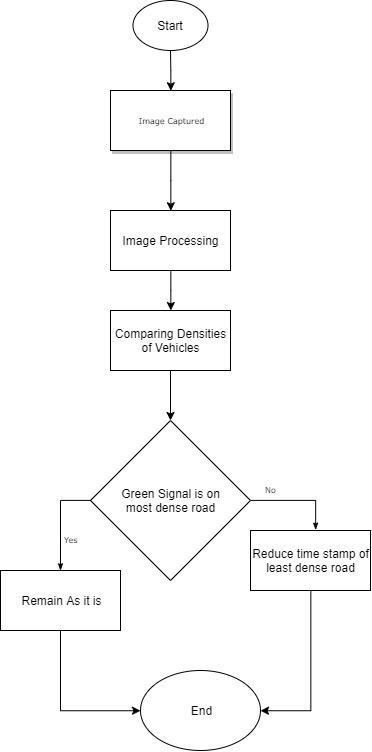
\includegraphics[scale=.40]{1.jpg}
\end{figure}

\pagebreak
\section*{Circuit Diagram}
\begin{figure}[!htb]
\begin{center}
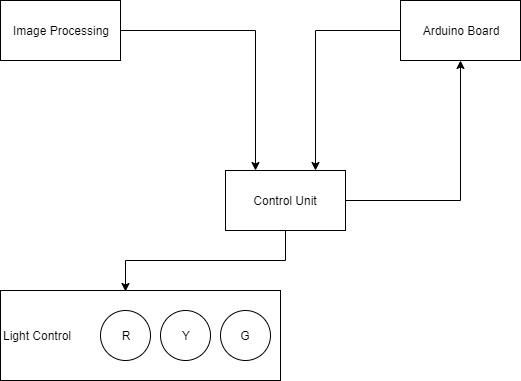
\includegraphics[scale=.45]{2.jpg}
\end{center}
\end{figure}

\pagebreak
\section*{Feasibility}
Three grain storage facilities are evaluated, a in-bin dryer storage system (dries and stores grain in bulk) and warehouse storage systems (grain is dried, and stored).
\\
It is one time investment.
\\
Prevents wastage and spoilage of grain upto 90-95%.
\\
It is cost efficient and does not harm any natural resources.


\section*{References:}
1.	http://www.iosrjournals.org/
\\
2.	https://www.newindianexpress.com/thesundaystandard/2018/mar/25/grain-drain
\\
3.	http://fci.gov.in/app2/webroot/upload/tenders/KD3Narela.pdf
\\
4.	https://blog.forumias.com/article/food-grain-storage-problem-in-india
\\
5.	https://msu.edu/~brook/publications/aeis/aeis647.htm 


\end{document}